% Provenance (never printed): old seconde/premiere S material on water as a
% resource (stocks and flows of the water cycle, residence times, groundwater,
% overuse as a physical fact); see sources/book2/PROVENANCE.md. Residence
% times are computed in figdata/grade-10/residence_times.py, the Aral Sea
% budget in figdata/grade-10/aral_sea.py.
\chapter{मीठे जल के संसाधन}\label{ch:g10:freshwater-resources}

1960 में मध्य एशिया के मरुस्थलों में स्थित अरल सागर संसार की चौथी सबसे बड़ी
झील था। दूर के पर्वतों की हिम और वर्षा से पोषित दो बड़ी नदियाँ
उसमें बहती थीं; उससे कोई नदी बाहर नहीं निकलती थी। 1960 के दशक में उनका जल
मरुस्थल की सिंचाई के लिए ले जाया गया। उपग्रहों ने देखा कि आगे क्या हुआ: झील
टुकड़ों में टूट गई है, और उसका अधिकांश तल अब सूखी भूमि है। इसका कारण
अत्यधिक रूप से जलवायु का परिवर्तन नहीं, बल्कि सिंचाई थी: झील को
हर वर्ष उससे कहीं कम जल मिला जितना वाष्पन उससे ले जाता था। यह अध्याय पृथ्वी के जल की गिनती करता है, कि वह कहाँ
संचित है और कितनी तेज़ी से चलता है, और दिखाता है कि जल का संसाधन सबसे
बढ़कर एक प्रवाह है: जब किसी जलाशय से उसमें आने वाले जल से अधिक लिया जाता है, तो
जलाशय खाली होता जाता है, उस दर से जिसका एक सरल बजट पूर्वानुमान करता है।
% ledger: nasa:aral, gaybullaev:aral-1960, micklin:aral

\begin{omfigure}
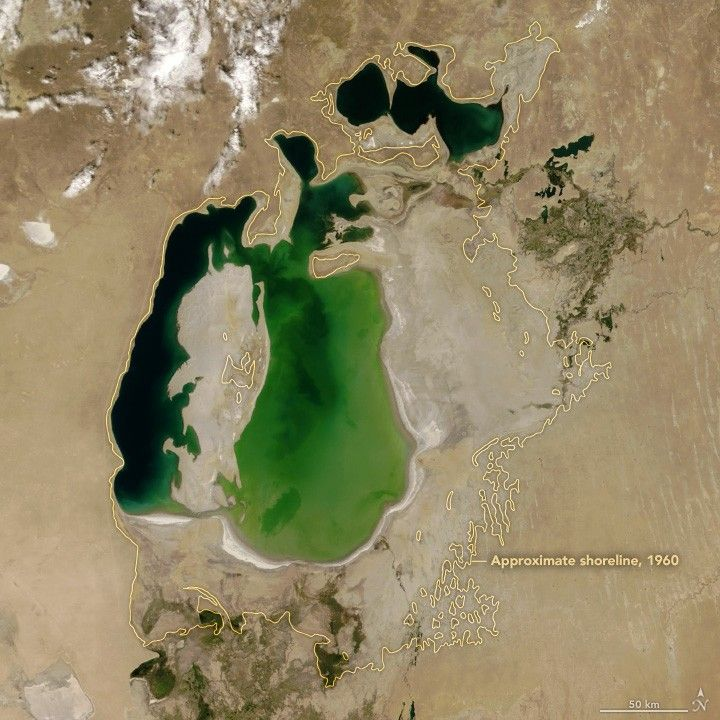
\includegraphics[width=0.47\linewidth]{images/book2/g10-nasa-aral-2000.jpg}\hspace{0.03\linewidth}%
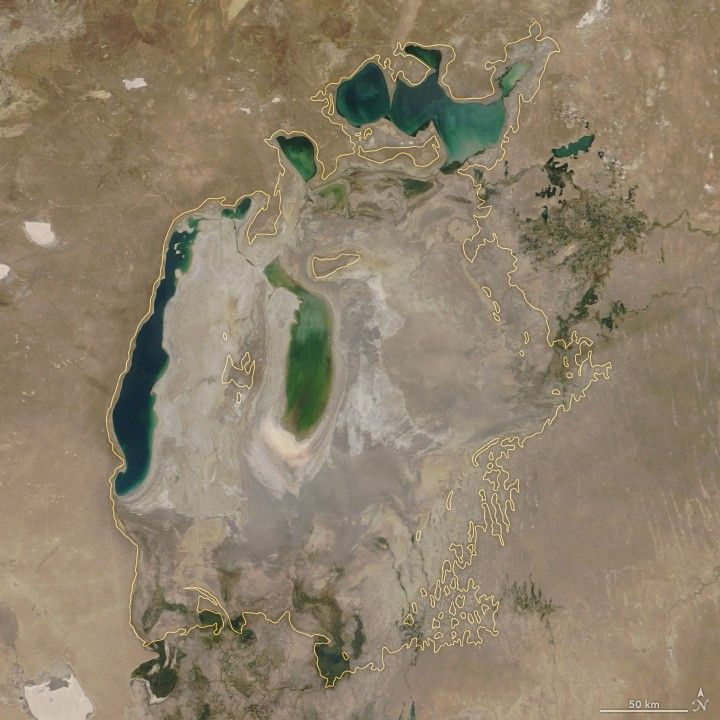
\includegraphics[width=0.47\linewidth]{images/book2/g10-nasa-aral-2018.jpg}

{\small NASA के टेरा उपग्रह पर लगे MODIS उपकरण द्वारा देखा गया अरल सागर,
अगस्त 2000 (बाएँ) और अगस्त 2018 (दाएँ); पीली रेखा 1960 की लगभग
तटरेखा है। पैमाना-पट्टी \qty{50}{km} की है। चित्र: NASA पृथ्वी
वेधशाला।}
\end{omfigure}

\begin{recall}
जल चक्र जल को महासागर, वायु और स्थल के बीच चलाता है:
वाष्पन, बादलों में संघनन, वर्षण, अपवाह; जल का कुल द्रव्यमान
संरक्षित रहता है (भौतिकी की पुस्तकें)। जुड़े हुए छिद्रों वाली चट्टानें
पारगम्य होती हैं; भौम जलस्तर के नीचे उनके छिद्र जल से भरे होते हैं, और ऐसी परत
जो कुओं को पोषित करने लायक़ पर्याप्त जल धारण करती और आगे जाने देती है, जलभृत है
(पुस्तक 1, कक्षा 6)। पृथ्वी का अधिकांश जल खारा जल है (पुस्तक 1,
कक्षा 2)। नदी अपनी \omterm{def:g10:drainage-basins:drainage-basin}{अपवाह द्रोणी} का जल बहा ले जाती है; उसका \omterm{def:g10:drainage-basins:discharge}{विसर्जन}
प्रति सेकंड आयतन है (\cref{ch:g10:drainage-basins})।
\end{recall}

\section{जल कहाँ है}

पृथ्वी में लगभग 1.39 अरब घन किलोमीटर जल है। इसका लगभग सारा
महासागर में है; केवल \qty{2.5}{\percent} मीठा है। और उस मीठे
जल का अधिकांश भाग पहुँच से बाहर है: इसका दो-तिहाई से अधिक हिम-टोपियों
और हिमनदों में जमा है, और लगभग एक-तिहाई भूमिगत है।
% ledger: usgs:water-stocks

\begin{center}
\small
\begin{tabular}{|l|r|r|}
\hline
\textbf{जलाशय} & \textbf{आयतन (\unit{km^3})} & \textbf{मीठे जल में अंश} \\ \hline
महासागर, समुद्र और खाड़ियाँ & \num{1338000000} & (खारा) \\ \hline
हिम-टोपियाँ, हिमनद और स्थायी हिम & \num{24064000} & \qty{68.7}{\percent} \\ \hline
मीठा भौम जल & \num{10530000} & \qty{30.1}{\percent} \\ \hline
भूमिगत बर्फ़ और पर्माफ़्रॉस्ट & \num{300000} & \qty{0.86}{\percent} \\ \hline
मीठे जल की झीलें & \num{91000} & \qty{0.26}{\percent} \\ \hline
मृदा की नमी & \num{16500} & \qty{0.05}{\percent} \\ \hline
वायुमंडल & \num{12900} & \qty{0.04}{\percent} \\ \hline
नदियाँ & \num{2120} & \qty{0.006}{\percent} \\ \hline
\end{tabular}

{\small संसार के जल का एक अनुमान, शिक्लोमानोव (1993) के अनुसार, अमेरिकी
भूवैज्ञानिक सर्वेक्षण से। खारा भौम जल (\num{12870000}~\unit{km^3}) और
खारी झीलें छोड़ दी गई हैं।}
\end{center}
% ledger: usgs:water-stocks

नदियाँ और मीठे जल की झीलें, जिनसे लोग अपने उपयोग का अधिकांश जल लेते हैं,
मिलकर सारे जल के एक प्रतिशत के सौवें भाग से भी कम रखती हैं। फिर भी
नदियाँ कभी देर तक सूखी नहीं रहतीं: वे \omterm{def:g10:freshwater-resources:stock}{भंडार} नहीं बल्कि प्रवाह हैं, जो हर
वर्षा से फिर भर जाती हैं।

\section{भंडार और अभिवाह}

\begin{definition}[भंडार; अभिवाह]\label{def:g10:freshwater-resources:stock}
जल के किसी बजट में \emph{भंडार}\index{भंडार (जल का)} किसी दिए हुए समय पर किसी
जलाशय --- महासागर, वायु, बर्फ़, कोई जलभृत, कोई
झील --- में रखे जल की मात्रा है, आयतन या द्रव्यमान के रूप में।
\emph{अभिवाह}\index{अभिवाह (जल का)} वह मात्रा है जो प्रति इकाई
समय एक जलाशय से दूसरे जलाशय में जाती है, उदाहरण के लिए घन किलोमीटर प्रति वर्ष में।
\end{definition}

\omterm{def:g10:freshwater-resources:stock}{भंडार} केवल अपने अभिवाहों के द्वारा बदलता है: जो आता है उसमें से जो जाता है। जब
दोनों बराबर हों, तो \omterm{def:g10:freshwater-resources:stock}{भंडार} \emph{स्थायी अवस्था} में होता है: वह वैसा ही रहता है,
यद्यपि उसका जल लगातार बदलता रहता है।

\begin{omfigure}
\begin{tikzpicture}[font=\footnotesize, >={Stealth[length=6pt]}]
  % ocean, land, atmosphere
  \fill[omSea] (0,0) rectangle (6.4,1.6);
  \fill[omLithAlluv] (6.4,0) -- (6.4,1.6) -- (8.2,2.1) -- (10.4,2.6) -- (12,2.9) -- (12,0) -- cycle;
  \fill[omLithSand!60] (6.4,0) -- (12,0) -- (12,1.0) -- (6.4,0.7) -- cycle;
  \draw[black!50] (6.4,1.6) -- (8.2,2.1) -- (10.4,2.6) -- (12,2.9);
  \fill[omIce] (10.6,2.65) -- (11.3,3.35) -- (12,2.9) -- cycle;
  \node[align=center] at (3.2,0.75) {\textbf{महासागर}\\\num{1335040}};
  \node[align=center] at (9.3,1.35) {मृदा की नमी 122\\झीलें और नदियाँ 178};
  \node[align=center] at (9.3,0.35) {भौम जल \num{15300}};
  \node[align=center] at (11.2,2.25) {बर्फ़\\\num{26350}};
  % atmosphere
  \draw[black!30, rounded corners=8pt, fill=omWxCloud] (1.0,4.6) rectangle (11.0,5.6);
  \node[align=center] at (6.0,5.1) {\textbf{वायुमंडल} 12.7};
  % fluxes
  \draw[->, omProp, line width=1.4pt] (1.4,1.7) -- node[left, align=right] {वाष्पन\\413} (1.4,4.5);
  \draw[->, omWxRain, line width=1.4pt] (4.4,4.5) -- node[pos=0.3, right, align=left] {वर्षण\\373} (4.4,1.7);
  \draw[->, omWxRain, line width=1.4pt] (7.6,4.5) -- node[pos=0.7, left, align=right] {वर्षण\\113} (7.6,2.05);
  \draw[->, omProp, line width=1.4pt] (10.0,2.6) -- node[right, align=left] {वाष्पन और\\वाष्पोत्सर्जन 73} (10.0,4.5);
  \draw[->, black!60, line width=1.2pt] (4.9,5.85) -- node[above] {स्थल के ऊपर ले जाई गई जलवाष्प: 40} (7.4,5.85);
  \draw[->, omRiver, line width=1.4pt] (7.6,1.2) -- node[above, inner sep=2pt] {अपवाह 40} (6.0,1.2);
\end{tikzpicture}

{\small 1990 के दशक का वैश्विक जल चक्र (व्यवस्था-चित्र; पैमाने पर नहीं)। \omterm{def:g10:freshwater-resources:stock}{भंडार}
हज़ार \unit{km^3} में, \omterm{def:g10:freshwater-resources:stock}{अभिवाह} हज़ार \unit{km^3} प्रति वर्ष में।
ट्रेनबर्थ और अन्य (2007) के अनुसार। भंडारों के अनुमान एक
अध्ययन से दूसरे में अलग होते हैं: यहाँ के भौम जल और बर्फ़ की तुलना ऊपर की तालिका से कीजिए।}
\end{omfigure}
% ledger: trenberth:water-cycle

चक्र संतुलित है। हर वर्ष महासागर वाष्पन द्वारा \num{413000}~\unit{km^3} खोता है
और \num{373000} वर्षा और हिम के रूप में तथा \num{40000} नदियों से
वापस पाता है। वायु $413\,000 + 73\,000 = \num{486000}$~\unit{km^3}
पाती है और $373\,000 + 113\,000$ लौटाती है, यानी उतना ही। स्थल
\num{113000}~\unit{km^3} वर्षण पाता है; \num{73000} वाष्पन द्वारा और पौधों की
पत्तियों से होकर वायु में लौट जाते हैं, और बाक़ी \num{40000}
नदियों में और भूमिगत होकर समुद्र तक बह जाते हैं।
% ledger: trenberth:water-cycle

\begin{definition}[नवीकरणीय मीठा जल]\label{def:g10:freshwater-resources:renewable}
किसी क्षेत्र का \emph{नवीकरणीय मीठा जल}\index{नवीकरणीय मीठा जल}
वर्षण द्वारा हर वर्ष नवीकृत मीठे जल का वह \omterm{def:g10:freshwater-resources:stock}{अभिवाह} है, जो
उसमें से नदियों में अपवाह के रूप में और भौम जल के रूप में बहता है। यह एक \omterm{def:g10:freshwater-resources:stock}{अभिवाह} है, घन
किलोमीटर प्रति वर्ष में, \omterm{def:g10:freshwater-resources:stock}{भंडार} नहीं।
\end{definition}

पृथ्वी के सारे स्थल के लिए यह वही \num{40000}~\unit{km^3} है जो हर वर्ष
समुद्र तक पहुँचता है। कोई क्षेत्र अपने नवीकरणीय जल का उपयोग वर्ष-दर-वर्ष
बिना कमी के कर सकता है। जो वह इससे अधिक लेता है, वह केवल किसी \omterm{def:g10:freshwater-resources:stock}{भंडार} से आ सकता है,
जो तब सिकुड़ता जाता है।

\section{निवास काल}

जल का एक अणु किसी जलाशय में कितनी देर रहता है? कुछ तुरंत निकल जाते हैं,
कुछ कहीं अधिक देर रहते हैं; पर औसत रूप से, उत्तर केवल \omterm{def:g10:freshwater-resources:stock}{भंडार} और
\omterm{def:g10:freshwater-resources:stock}{अभिवाह} से निकल आता है।

\begin{definition}[निवास काल]\label{def:g10:freshwater-resources:residence-time}
किसी जलाशय में जल का \emph{निवास काल}\index{निवास काल} वह
औसत समय है जो जल उसमें प्रवेश करने और निकलने के बीच बिताता है।
\end{definition}

\begin{proposition}[निवास काल, भंडार और अभिवाह]\label{prop:g10:freshwater-resources:residence}
स्थायी अवस्था में किसी ऐसे जलाशय के लिए, जिसमें \omterm{def:g10:freshwater-resources:stock}{भंडार} $S$ है और जिससे \omterm{def:g10:freshwater-resources:stock}{अभिवाह} $F$
(भीतर और बाहर) गुज़रता है, \omterm{def:g10:freshwater-resources:residence-time}{निवास काल} यह है:
\[
T = \frac{S}{F}.
\]
\end{proposition}

\begin{proof}
स्थायी अवस्था में हर वर्ष आयतन $F$ प्रवेश करता है और आयतन $F$ निकलता है, जबकि
\omterm{def:g10:freshwater-resources:stock}{भंडार} $S$ बना रहता है। समय $S/F$ के बाद आयतन $F \times S/F = S$
प्रवेश कर चुका होता है: उतना जितना पूरा जलाशय धारण करता है। औसत रूप से, आरंभ में
उपस्थित जल तब तक बदल चुका होता है, इसलिए जल जलाशय में $S/F$ समय रहता है।
\end{proof}

\begin{example}[वायु में जल]\label{ex:g10:freshwater-resources:atmosphere}
वायुमंडल \num{12700}~\unit{km^3} जल धारण करता है, और
हर वर्ष उसमें से \num{486000}~\unit{km^3} वर्षा और हिम के रूप में गिरता है। उसका
\omterm{def:g10:freshwater-resources:residence-time}{निवास काल} $12\,700/486\,000 \approx \num{0.026}$ वर्ष है, यानी लगभग
\num{9.5} दिन: वायु का जल हर एक-दो सप्ताह में नवीकृत हो जाता है। आज बरसने वाला
बादल ऐसे जल से बना है जो कुछ दिन पहले महासागर या ज़मीन से
निकला था।
\end{example}
% ledger: trenberth:water-cycle (t_atmosphere_days 9.5 in figdata/grade-10/residence_times.py)

यही परिकलन नदी की धाराओं के जल के लिए लगभग \num{19} दिन देता है
($2120$~\unit{km^3}, जिन्हें प्रति वर्ष \num{40000}~\unit{km^3} बहा ले जाते हैं), झीलों और नदियों को
मिलाकर कुछ वर्ष, और महासागर के लिए लगभग \num{3200} वर्ष
($1\,335\,040/413$ हज़ार~\unit{km^3})। भौम जल इससे भी धीमा हो सकता है:
कुछ जलभृतों का सबसे गहरा जल लाखों वर्ष पुराना है।
% ledger: trenberth:water-cycle, usgs:water-stocks, sturchio:nubian-age

\begin{omfigure}
\begin{tikzpicture}
\begin{axis}[omrecord, xbar, xmode=log, log origin=infty, width=0.74\linewidth, height=5.6cm,
  xmin=1, xmax=1e9, ymin=-0.6, ymax=4.6, bar width=11pt,
  ytick={0,1,2,3,4}, yticklabels={वायुमंडल, नदियाँ, {झीलें और नदियाँ}, महासागर, {गहरा भौम जल (आयु)}},
  xtick={1,30.44,365.25,36525,3652500,365250000}, xticklabels={1 दिन, 1 महीना, 1 वर्ष, 100 वर्ष, \num{10000} वर्ष, 1 मिलियन वर्ष},
  xticklabel style={font=\scriptsize, rotate=25, anchor=north east}, yticklabel style={font=\small},
  xlabel={निवास काल (लघुगणकीय पैमाना)}, label style={font=\small}, xmajorgrids]
\addplot[fill=omDef!45, draw=omDef!80!black] table[x=days, y=idx] {figdata/out/grade-10-residence_times-times.dat};
\draw[fill=omProp!45, draw=omProp!80!black] (axis cs:73050000,3.75) rectangle (axis cs:365250000,4.25);
\node[anchor=west, font=\scriptsize] at (axis cs:9.5,0) {\num{9.5} दिन};
\node[anchor=west, font=\scriptsize] at (axis cs:19.4,1) {\num{19} दिन};
\node[anchor=west, font=\scriptsize] at (axis cs:1625,2) {\num{4.5} वर्ष};
\node[anchor=west, font=\scriptsize] at (axis cs:1180690,3) {\num{3200} वर्ष};
\node[anchor=east, font=\scriptsize] at (axis cs:73050000,4) {\num{200000} से 1 मिलियन वर्ष};
\end{axis}
\end{tikzpicture}

{\small जल के \omterm{def:g10:freshwater-resources:residence-time}{निवास काल}, वैश्विक जल चक्र से \omterm{def:g10:freshwater-resources:stock}{भंडार} को \omterm{def:g10:freshwater-resources:stock}{अभिवाह} से भाग देकर
परिकलित (नीला), और पूर्वी सहारा के नीचे के गहरे भौम जल की मापी गई आयु
(नारंगी)। लघुगणकीय अक्ष: एक वर्ष से आगे हर अंकित चरण सौ गुना है। आँकड़े:
ट्रेनबर्थ और अन्य (2007); अमेरिकी भूवैज्ञानिक सर्वेक्षण; स्टर्चियो और अन्य
(2004)।}
\end{omfigure}
% values computed in figdata/grade-10/residence_times.py

\omterm{def:g10:freshwater-resources:residence-time}{निवास काल} मापता है कि कोई जलाशय कितनी तेज़ी से सँभलता है। नदी से लिया गया जल
दिनों में बदल जाता है; प्रदूषित या खाली हुई झील को वर्ष लगते हैं; जिस भौम जल
को एकत्र होने में हज़ारों वर्ष लगे, वह मानव जीवन के पैमाने पर बिल्कुल
नवीकृत नहीं होता।

\begin{method}[जल का बजट]\label{met:g10:freshwater-resources:budget}
\begin{enumerate}
  \item जलाशय चुनिए: कोई झील, कोई जलभृत, कोई द्रोणी, वायु।
  \item उसमें आने वाले हर \omterm{def:g10:freshwater-resources:stock}{अभिवाह} (नदियाँ, वर्षा, रिसाव) और उससे जाने वाले हर \omterm{def:g10:freshwater-resources:stock}{अभिवाह}
        (नदियाँ, वाष्पन, पंपिंग) की सूची, एक ही इकाई में, बनाइए।
  \item \omterm{def:g10:freshwater-resources:stock}{भंडार} में प्रति वर्ष परिवर्तन आगतों के योग में से निर्गतों के
        योग को घटाने पर मिलता है।
  \item यदि \omterm{def:g10:freshwater-resources:stock}{भंडार} नहीं बदलता, तो आगत निर्गतों के बराबर हैं, और \omterm{def:g10:freshwater-resources:residence-time}{निवास
        काल} \omterm{def:g10:freshwater-resources:stock}{भंडार} को इनमें से किसी से भी भाग देने पर मिलता है।
\end{enumerate}
\end{method}

\section{जलाशयों के रूप में जलभृत}

ज़मीन में रिसकर भौम जलस्तर तक पहुँचने वाली वर्षा नीचे के जलभृत का
\emph{पुनर्भरण} करती है। फिर जल चट्टान के छिद्रों से होकर धीरे-धीरे
सोतों, नदियों या समुद्र की ओर चलता है। जहाँ कोई
पारगम्य परत किसी अपारगम्य परत, जैसे चिकनी मिट्टी, के नीचे झुकती है, वहाँ उसका जल
\emph{परिरुद्ध} होता है: उसे केवल वहीं पोषण मिलता है जहाँ परत सतह तक पहुँचती है, जो
बहुत दूर हो सकता है।

\begin{omfigure}
\begin{tikzpicture}[font=\footnotesize, >={Stealth[length=5pt]}]
  % layers dipping to the right
  \fill[lith shale] (0,0) -- (12,0) -- (12,0.8) -- (0,2.4) -- cycle;
  \fill[lith sandstone] (0,2.4) -- (12,0.8) -- (12,2.2) -- (2.2,3.5) -- (0,3.8) -- cycle;
  \fill[lith shale] (2.2,3.5) -- (12,2.2) -- (12,3.4) -- (3.6,3.9) -- cycle;
  % ground surface
  \draw[line width=0.8pt, brown!60!black] (0,3.8) -- (1.2,4.0) -- (2.2,3.9) -- (3.6,3.9) -- (6,3.6) -- (9,3.5) -- (12,3.4);
  \fill[omLithAlluv] (0,3.8) -- (1.2,4.0) -- (2.2,3.9) -- (2.2,3.5) -- (0,3.8) -- cycle;
  \fill[omLithAlluv] (2.2,3.9) -- (3.6,3.9) -- (2.2,3.5) -- cycle;
  \fill[omLithAlluv] (3.6,3.9) -- (6,3.6) -- (9,3.5) -- (12,3.4) -- (3.6,3.9) -- cycle;
  % water table in the unconfined part
  \draw[omDef, line width=1pt, dashed] (0,3.3) .. controls (1.0,3.35) and (1.8,3.2) .. (2.6,3.45);
  \node[anchor=south west, text=omDef, fill=white, fill opacity=0.8, text opacity=1, inner sep=1pt] at (0.05,2.75) {भौम जलस्तर};
  % rain and recharge
  \foreach \x in {0.35,0.65,0.95,1.25} \draw[omWxRain, thick] (\x,4.9) -- (\x-0.15,4.4);
  \node[anchor=south, text=omWxRain] at (0.7,4.95) {वर्षा: पुनर्भरण};
  % flow arrows in the aquifer
  \draw[->, omDef, line width=1.1pt] (2.0,2.85) -- (4.4,2.55);
  \draw[->, omDef, line width=1.1pt] (5.4,2.4) -- (7.8,2.1);
  \draw[->, omDef, line width=1.1pt] (8.8,1.95) -- (11.2,1.65);
  % wells
  \draw[black!70, line width=1.6pt] (1.95,3.95) -- (1.95,2.9);
  \node[anchor=south] at (1.95,4.0) {कुआँ};
  \draw[black!70, line width=1.6pt] (7.0,3.55) -- (7.0,1.9);
  \node[anchor=south] at (7.0,3.6) {कुआँ};
  % labels
  \node[align=center, fill=white, fill opacity=0.85, text opacity=1, inner sep=1.5pt] at (1.5,0.8) {अपारगम्य चिकनी मिट्टी};
  \node[align=center, fill=white, fill opacity=0.85, text opacity=1, inner sep=1.5pt] at (8.6,2.95) {अपारगम्य चिकनी मिट्टी};
  \node[anchor=north, align=center] at (1.6,-0.1) {अपरिरुद्ध जलभृत:\\पुनर्भरण क्षेत्र};
  \node[anchor=north, align=center] at (6.4,-0.1) {परिरुद्ध जलभृत};
  \node[anchor=north, align=center] at (10.6,-0.1) {पुराना जल, पुनर्भरण\\क्षेत्र से दूर};
\end{tikzpicture}

{\small एक पारगम्य बलुआ पत्थर में एक जलभृत (व्यवस्था-चित्र)। जहाँ यह सतह तक
पहुँचता है वहाँ वर्षा इसका पुनर्भरण करती है; वहाँ भौम जलस्तर चढ़ने-उतरने के लिए स्वतंत्र है।
आगे, चिकनी मिट्टी के नीचे, जलभृत परिरुद्ध है, और उसका जल परत में नीचे की ओर
धीरे-धीरे चलता है: पुनर्भरण क्षेत्र से जितना दूर, जल उतना ही
पुराना।}
\end{omfigure}

\begin{definition}[जीवाश्म भौम जल]\label{def:g10:freshwater-resources:fossil-groundwater}
\emph{जीवाश्म भौम जल}\index{जीवाश्म भौम जल} ऐसा भौम जल है जो
बहुत पहले, प्रायः किसी अधिक आर्द्र जलवायु में, अपने जलभृत में प्रवेश कर चुका था, और जिसे आज का
पुनर्भरण मानव जीवनकाल के पैमाने पर नवीकृत नहीं करता।
\end{definition}

पूर्वी सहारा के नीचे बलुआ पत्थर का एक विशाल जलभृत है। उसका सबसे गहरा जल,
जिसकी आयु क्रिप्टॉन के एक दुर्लभ रेडियोधर्मी रूप के क्षय से निकाली गई है,
\num{200000} से एक मिलियन वर्ष पुराना है। यह दक्षिण-पश्चिमी मिस्र के एक पुनर्भरण क्षेत्र से
धीरे-धीरे भीतर बहकर आया, और इसका रसायन दिखाता है कि यह हिमयुगों के
पिछले आर्द्र कालों में वर्षा के रूप में गिरा था, जब अटलांटिक से नम हवा
इस क्षेत्र तक पहुँचती थी। आज पंप किया गया ऐसा जल खनन किया जा रहा \omterm{def:g10:freshwater-resources:stock}{भंडार} है, प्रवाह नहीं।
% ledger: sturchio:nubian-age

जब पंपिंग पुनर्भरण से अधिक होती है, तो भौम जलस्तर गिरता है। मध्य संयुक्त राज्य अमेरिका के
हाई प्लेन्स में लगभग \num{175000} वर्ग मील
(\qty{453000}{km^2}) के नीचे के जलभृत को लगभग 1950 से सिंचाई के लिए पंप किया गया है। 2015 तक
उसका जल-तल औसतन \qty{4.8}{m} गिर चुका था, और कुछ कुओं में
\qty{71}{m} (234 फ़ुट) तक; जलभृत लगभग
\num{273} मिलियन एकड़-फ़ुट, यानी लगभग \qty{340}{km^3}, जल खो चुका था।
% ledger: mcguire:high-plains (1 acre-foot = 1233.5 m3)

\begin{omfigure}
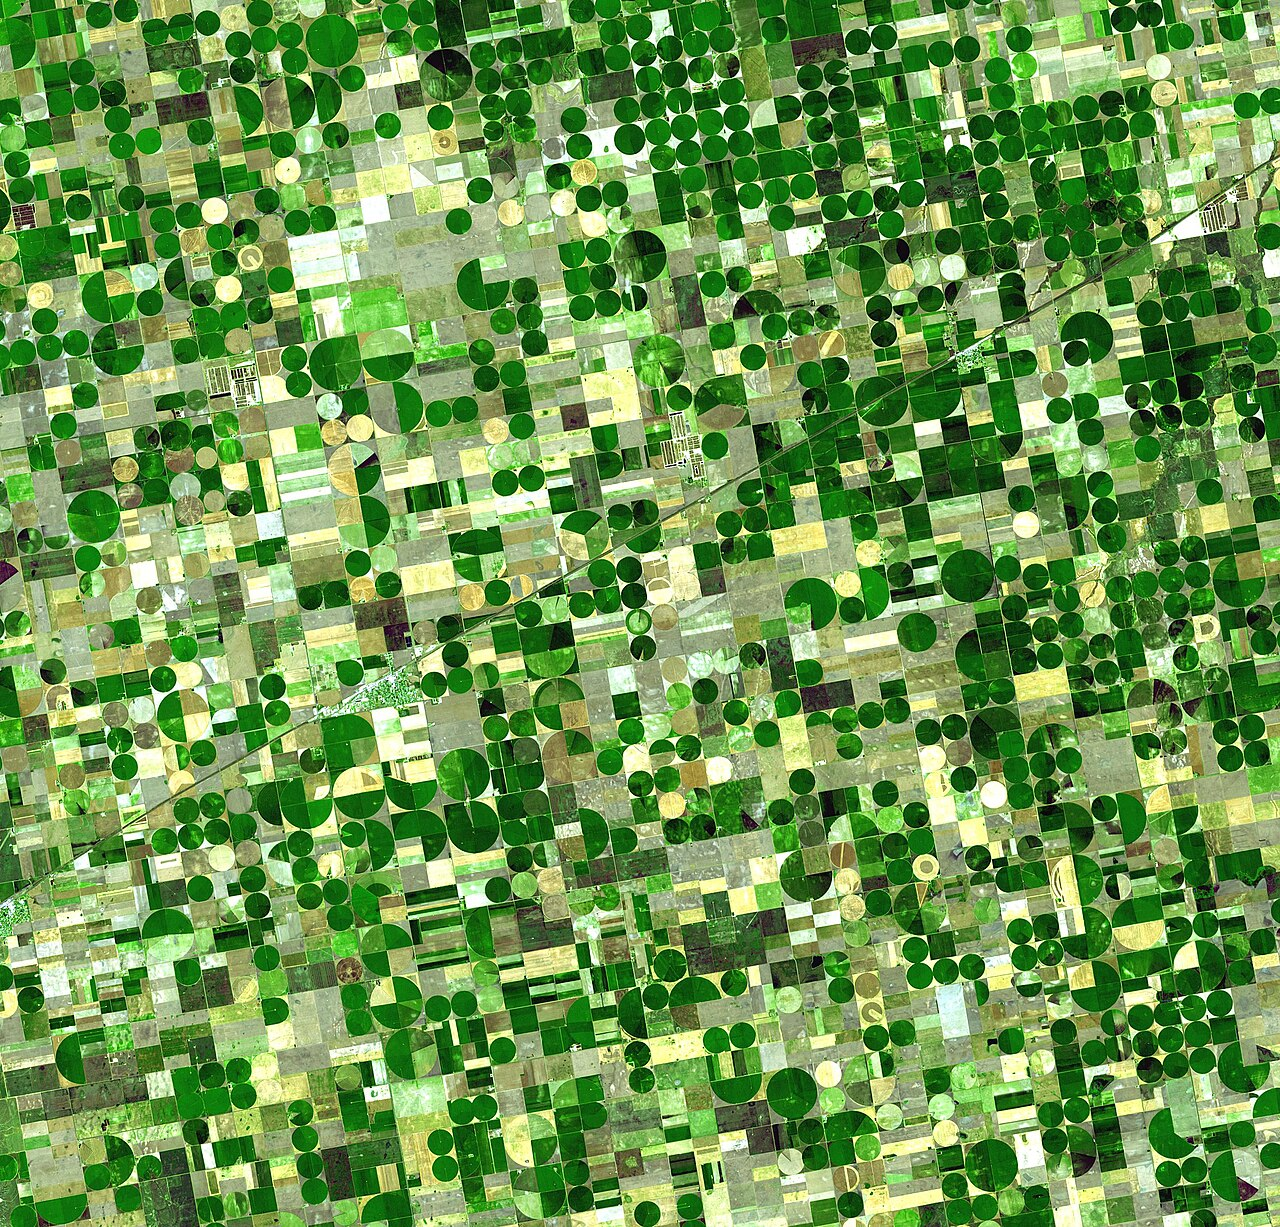
\includegraphics[width=0.5\linewidth]{images/book2/g10-nasa-kansas-center-pivot.jpg}

{\small सबलेट, कैनसस, के पास सिंचित खेत, जिन्हें जून 2001 में NASA के टेरा उपग्रह पर लगे ASTER उपकरण ने
देखा (लगभग \qty{37}{km} चौड़ा क्षेत्र)। हर वृत्त
एक खेत है जिसे अपने केंद्र के चारों ओर घूमती एक लंबी छिड़काव-भुजा सींचती है;
वृत्त \num{800} और \qty{1600}{m} चौड़े हैं। चित्र: NASA (सार्वजनिक डोमेन)।}
\end{omfigure}

भौम जल अंतरिक्ष से देखा नहीं जा सकता, पर तौला जा सकता है: एक के पीछे एक उड़ते
दो उपग्रह पृथ्वी के खिंचाव में उन हल्के परिवर्तनों को महसूस करते हैं जो
उनके नीचे आते-जाते जल के द्रव्यमान से होते हैं, और मानचित्र बनाते हैं कि स्थल पर जल का \omterm{def:g10:freshwater-resources:stock}{भंडार}
महीने-दर-महीने कहाँ बढ़ता और घटता है।

\begin{omfigure}
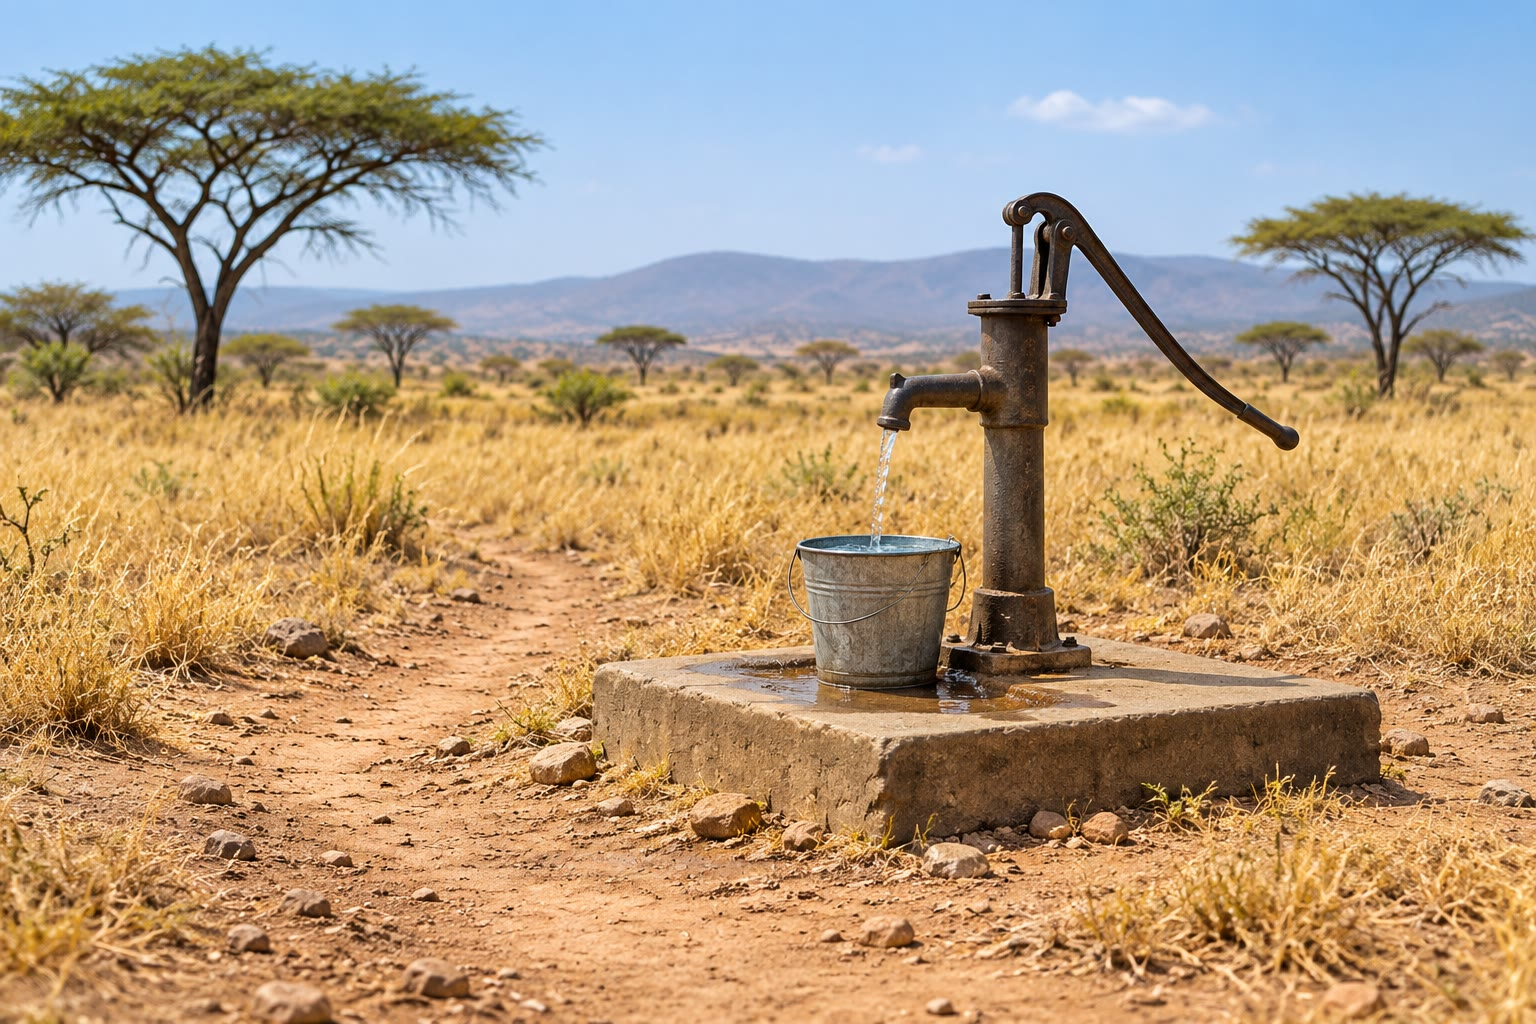
\includegraphics[width=0.55\linewidth]{images/book2/ai/g10-hand-pump-well.jpg}

{\small एक शुष्क भूदृश्य में किसी कुएँ पर एक हैंडपंप: यहाँ खींचा गया जल
नीचे की ज़मीन से आता है, शुष्क ऋतु की पहुँच से बाहर।}
\end{omfigure}

\section{भौतिक तथ्य के रूप में अति-उपयोग}

अरल सागर का कोई निकास नहीं है: उसकी दो नदियों, अमु दरिया और
सिर दरिया, का जल केवल वाष्पन से निकलता है। 1960 में यह
\qty{68000}{km^2} में फैला था, \qty{1093}{km^3} जल रखता था और इसके जल में प्रति लीटर \qty{10}{g}
लवण था। उस वर्ष वाष्पन ने \qty{71.1}{km^3} निकाला, और झील पर हुई वर्षा
\qty{9.4}{km^3} लाई: अपना तल बनाए रखने के लिए झील को अपनी नदियों से
प्रति वर्ष $71.1 - 9.4 = \qty{61.7}{km^3}$ चाहिए था।
% ledger: gaybullaev:aral-1960, gaybullaev:aral-table

1960 के दशक से नदियों को मरुस्थल की सिंचाई के लिए मोड़ दिया गया, और उनका लगभग
कोई भी जल झील तक नहीं पहुँचा: 1970 और 1980 के दशकों में प्रायः
प्रति वर्ष \qty{2}{km^3} से कम। वाष्पन चलता रहा, और झील
सिकुड़ने लगी। उसका बजट तय करता है कि कितनी तेज़ी से। वाष्पन जल की ऐसी परत ले जाता है
जिसकी मोटाई जलवायु पर निर्भर करती है, यहाँ लगभग एक मीटर प्रति वर्ष
($71.1/68\,000 \approx \qty{0.00105}{km}$)। यदि अंतर्वाह रुक जाए, तो तल
हर वर्ष लगभग इतना गिरता है, वर्षा घटाकर। झील के सिकुड़ने के साथ उसका
क्षेत्रफल और इसलिए उसका वाष्पन भी सिकुड़ता है, और गिरावट धीमी हो जाती है; पर वह
तब तक नहीं रुकती जब तक अंतर्वाह और वाष्पन फिर से संतुलित न हो जाएँ।
% ledger: gaybullaev:aral-table (values computed in figdata/grade-10/aral_sea.py)

\begin{omfigure}
\begin{tikzpicture}
\begin{axis}[omrecord, name=vol, width=0.46\linewidth, height=5.4cm, xmin=1955, xmax=2012, ymin=0, ymax=1200,
  xtick={1960,1980,2000}, xticklabel style={/pgf/number format/1000 sep={}}, scaled y ticks=false,
  ylabel={आयतन (\unit{km^3})}, xlabel={वर्ष}, tick label style={font=\small}, label style={font=\small},
  title={\small जल का आयतन}]
\addplot[omDef, line width=1pt, mark=*, mark size=1.3pt] table[x=year, y=volume] {figdata/out/grade-10-aral_sea-record.dat};
\end{axis}
\begin{axis}[omrecord, at={(vol.east)}, anchor=west, xshift=1.4cm, width=0.46\linewidth, height=5.4cm,
  xmin=1955, xmax=2012, ymin=0, ymax=140, xtick={1960,1980,2000},
  xticklabel style={/pgf/number format/1000 sep={}},
  ylabel={लवणता (\unit{g/L})}, xlabel={वर्ष}, tick label style={font=\small}, label style={font=\small},
  title={\small लवणता}]
\addplot[omProp, line width=1pt, mark=*, mark size=1.3pt] table[x=year, y=salinity] {figdata/out/grade-10-aral_sea-record.dat};
\end{axis}
\end{tikzpicture}

{\small 1960 से 2010 तक अरल सागर: उसके जल का आयतन घटकर दसवाँ भाग
रह गया, जबकि वाष्पन द्वारा पीछे छोड़ा गया लवण तेरह गुना अधिक
सांद्र हो गया। आँकड़े: गायबुल्लाएव और अन्य (2012)।}
\end{omfigure}
% ledger: gaybullaev:aral-table

2010 तक झील में \qty{98}{km^3} जल था, जो उसके 1960 के आयतन का दसवाँ भाग था, और वह
\qty{14280}{km^2} में फैली थी; उसकी लवणता \qty{130}{g/L} तक पहुँच चुकी थी, जो महासागर से
कहीं अधिक खारी है। उसका तल \qty{20}{m} से अधिक गिर चुका था। सूखे तल से लवणीय धूल
उड़ती है। कारण छिपा नहीं है: झील का अंतर्वाह काट दिया गया
जबकि उसका वाष्पन नहीं कटा।
% ledger: gaybullaev:aral-table, gaybullaev:aral-1960, micklin:aral, nasa:aral

\section{अभ्यास}

\begin{exercise}[$\star$]\label{exo:g10:freshwater-resources:1}
\omterm{def:g10:freshwater-resources:stock}{भंडार}, \omterm{def:g10:freshwater-resources:stock}{अभिवाह} और \omterm{def:g10:freshwater-resources:residence-time}{निवास काल} की परिभाषा दीजिए, और हर एक की इकाइयाँ बताइए।
\end{exercise}

\begin{exercise}[$\star$]\label{exo:g10:freshwater-resources:2}
संसार के जल की तालिका से: सारे जल का कितना अंश मीठा है? मीठे
जल के कितने अंश जमे हुए और भूमिगत हैं? कौन-सा जलाशय सबसे
कम जल रखता है?
\end{exercise}

\begin{exercise}[$\star$]\label{exo:g10:freshwater-resources:3}
\omterm{def:g10:freshwater-resources:renewable}{नवीकरणीय मीठे जल} और \omterm{def:g10:freshwater-resources:fossil-groundwater}{जीवाश्म भौम जल} की परिभाषा दीजिए। पहला \omterm{def:g10:freshwater-resources:stock}{अभिवाह}
और दूसरा \omterm{def:g10:freshwater-resources:stock}{भंडार} क्यों है?
\end{exercise}

\begin{exercise}[$\star$]\label{exo:g10:freshwater-resources:4}
संसार की मीठे जल की झीलें (\num{91000}~\unit{km^3}) उसकी नदियों (\num{2120}~\unit{km^3})
से कितने गुना अधिक जल रखती हैं?
\end{exercise}

\begin{exercise}[$\star$]\label{exo:g10:freshwater-resources:5}
\omterm{def:g10:freshwater-resources:residence-time}{निवास कालों} के आरेख पर कौन-सा जलाशय अपना जल सबसे तेज़ी से नवीकृत करता है,
और कौन-सा सबसे धीरे? जल महासागर में वायु की तुलना में कितने गुना अधिक देर
रहता है?
\end{exercise}

\begin{exercise}[$\star\star$]\label{exo:g10:freshwater-resources:6}
वायुमंडल \num{12700}~\unit{km^3} जल रखता है। उसमें प्रवेश करने वाले वाष्पन
(हर वर्ष महासागर से \num{413000} और स्थल से \num{73000}~\unit{km^3}) से उसका \omterm{def:g10:freshwater-resources:residence-time}{निवास
काल} परिकलित कीजिए, और जाँचिए कि यह उससे बाहर निकलने वाले वर्षण से परिकलित \omterm{def:g10:freshwater-resources:residence-time}{निवास काल}
से मेल खाता है।
\end{exercise}

\begin{exercise}[$\star\star$]\label{exo:g10:freshwater-resources:7}
महासागर \num{1335040} हज़ार~\unit{km^3} जल रखता है और
वाष्पन द्वारा प्रति वर्ष \num{413} हज़ार~\unit{km^3} खोता है। उसका \omterm{def:g10:freshwater-resources:residence-time}{निवास
काल} परिकलित कीजिए। उसमें प्रवेश करने वाले जल से परिकलित करने पर यह वही क्यों रहता है?
\end{exercise}

\begin{exercise}[$\star\star$]\label{exo:g10:freshwater-resources:8}
वैश्विक जल चक्र के अभिवाहों की सहायता से स्थल का बजट लिखिए: उस पर क्या
गिरता है, क्या वायु में लौटता है, क्या बह जाता है। स्थल पर गिरने वाली वर्षा का
कितना अंश वायु में लौटता है?
\end{exercise}

\begin{exercise}[$\star\star$]\label{exo:g10:freshwater-resources:9}
हाई प्लेन्स जलभृत ने लगभग 1950 से 2015 तक लगभग \num{273.2} मिलियन एकड़-फ़ुट जल
खोया (\num{1}~एकड़-फ़ुट = \qty{1233.5}{m^3})। इस आयतन को
\unit{km^3} में बदलिए और इसकी तुलना 1987 में अरल सागर के आयतन
(\qty{345.6}{km^3}) से कीजिए।
\end{exercise}

\begin{exercise}[$\star\star$]\label{exo:g10:freshwater-resources:10}
हाई प्लेन्स जलभृत का औसत जल-तल लगभग 1950 से 2015 तक \num{15.8} फ़ुट
गिरा (\num{1}~फ़ुट = \qty{0.3048}{m})। यह मीटर में कितना है,
और सेंटीमीटर प्रति वर्ष में?
\end{exercise}

\begin{exercise}[$\star\star$]\label{exo:g10:freshwater-resources:11}
एक जलभृत \qty{2}{km^3} जल रखता है और उसका पुनर्भरण
प्रति वर्ष \qty{0.01}{km^3} होता है। उसके जल का \omterm{def:g10:freshwater-resources:residence-time}{निवास काल} क्या है? कुएँ अब
उससे प्रति वर्ष \qty{0.05}{km^3} पंप करते हैं। मान लीजिए कि पुनर्भरण चलता रहता है और
अब कुएँ ही जल के निकलने का एकमात्र रास्ता हैं: वह कितने समय
टिकेगा?
\end{exercise}

\begin{exercise}[$\star\star\star$]\label{exo:g10:freshwater-resources:12}
1960 में (\qty{1093}{km^3}, वाष्पन प्रति वर्ष \qty{71.1}{km^3}) और 2010 में
(\qty{98.1}{km^3}, वाष्पन प्रति वर्ष \qty{11.4}{km^3}) अरल सागर के जल का \omterm{def:g10:freshwater-resources:residence-time}{निवास काल}
परिकलित कीजिए। उसका
वाष्पन क्यों घटा?
\end{exercise}

\begin{exercise}[$\star\star\star$]\label{exo:g10:freshwater-resources:13}
बिना निकास की एक झील \qty{100}{km^2} में फैली है। वाष्पन उसकी सतह से प्रति वर्ष
\qty{1.2}{m} जल निकालता है, और वर्षा \qty{0.2}{m} जोड़ती है।
\begin{enumerate}
  \item कितना अंतर्वाह, \unit{km^3} प्रति वर्ष में, उसका तल स्थिर रखता है?
  \item अंतर्वाह आधा कर दिया जाता है। पहले वर्ष में तल कितना
        गिरता है?
  \item आगे के वर्षों में गिरावट धीमी क्यों हो जाती है?
\end{enumerate}
\end{exercise}

\begin{exercise}[$\star\star\star$]\label{exo:g10:freshwater-resources:14}
किसी मरुस्थल में वर्षा एक जलभृत का प्रति वर्ष \qty{1}{mm} जल से पुनर्भरण करती है।
जलभृत \qty{100}{m} मोटा है और जल उसके आयतन का \qty{20}{\percent} भरता
है। पुनर्भरण को इसे भरने में कितना समय लगेगा? इसकी तुलना
सहारा जलभृत के गहरे जल की आयु से कीजिए।
\end{exercise}

\begin{exercise}[$\star\star\star$]\label{exo:g10:freshwater-resources:15}
हाई प्लेन्स जलभृत लगभग \qty{453000}{km^2} में फैला है और 2015 तक लगभग
\qty{337}{km^3} जल खो चुका था। पूरे जलभृत पर फैलाने पर यह जल की कितनी
मोटाई है? उसका जल-तल औसतन \qty{4.8}{m} गिरा।
जल-तल की गिरावट खोए गए जल की मोटाई से अधिक क्यों है?
\end{exercise}

\section{समस्या: अरल सागर का बजट}

\begin{problem}[{सप्ताहांत समस्या --- कोई झील कितनी तेज़ी से लुप्त होती है?}]
\label{pb:g10:freshwater-resources:1}
% ledger: gaybullaev:aral-table, gaybullaev:aral-1960, micklin:aral (values computed in figdata/grade-10/aral_sea.py)
तालिका चार वर्षों के लिए अरल सागर का बजट देती है (आयतन
\unit{km^3} में, लवणता प्रति लीटर लवण के ग्राम में)। 1960 में झील
\qty{68000}{km^2} में फैली थी।
\begin{center}
\small
\begin{tabular}{|c|c|c|c|c|c|}
\hline
वर्ष & नदी-अंतर्वाह & झील पर वर्षा & वाष्पन & आयतन & लवणता \\ \hline
1960 & 42.0 & 9.4 & 71.1 & 1093.0 & 10.0 \\ \hline
1984 & 0.3 & 3.5 & 47.9 & 502.7 & 21.9 \\ \hline
1987 & 1.0 & 6.2 & 36.8 & 345.6 & 25.0 \\ \hline
1989 & 3.1 & 5.3 & 35.3 & 327.2 & 30.0 \\ \hline
\end{tabular}

{\small आँकड़े: गायबुल्लाएव और अन्य (2012)।}
\end{center}

\medskip
\noindent\textbf{भाग I --- 1960 में झील।}
\begin{enumerate}
  \item 1960 में झील की माध्य गहराई क्या थी?
  \item उसका आयतन घन मीटर में व्यक्त कीजिए।
  \item उसमें कितना लवण था, टन में?
  \item वाष्पन से गिनने पर उसके जल का \omterm{def:g10:freshwater-resources:residence-time}{निवास काल} क्या था?
  \item बिना निकास की झील केवल वाष्पन (और
        रिसाव) से ही जल क्यों खो सकती है?
\end{enumerate}

\medskip
\noindent\textbf{भाग II --- झील को क्या चाहिए।}
\begin{enumerate}[resume]
  \item 1960 में वाष्पन ने झील से जल की कितनी मोटी परत निकाली,
        मीटर में?
  \item वर्षा ने कितनी मोटाई जोड़ी?
  \item कितना नदी-अंतर्वाह वाष्पन और वर्षा को ठीक संतुलित कर देता?
  \item दोनों नदियाँ पर्वतों से औसतन प्रति वर्ष लगभग \qty{79}{km^3} और
        \qty{37}{km^3} बाहर लाती हैं। झील को इसका कितना अंश
        चाहिए होता?
\end{enumerate}

\medskip
\noindent\textbf{भाग III --- 1980 के दशक के अंत में झील।}
\begin{enumerate}[resume]
  \item 1987 का बजट लिखिए: आगत, निर्गत, शुद्ध परिवर्तन।
  \item 1984 और 1989 के बीच आयतन \qty{502.7}{km^3} से घटकर
        \qty{327.2}{km^3} रह गया। प्रति वर्ष औसत गिरावट क्या थी? इसकी तुलना
        1987 के बजट से कीजिए।
  \item मान लीजिए कि झील का एक वर्ग किलोमीटर वाष्पन द्वारा उतना ही जल खोता है
        जितना 1960 में। 1987 में झील का क्षेत्रफल क्या था?
  \item यह उसके 1960 के क्षेत्रफल का कितना अंश है?
  \item वाष्पन \qty{71.1}{km^3} से घटकर
        \qty{36.8}{km^3} क्यों रह गया था?
  \item 1987 में झील में उसके 1960 के आयतन का कितना अंश बचा था?
\end{enumerate}

\medskip
\noindent\textbf{भाग IV --- लवण और तल।}
\begin{enumerate}[resume]
  \item यदि 1960 का सारा लवण जल में ही रहा होता, तो 1987 में
        लवणता क्या होती?
  \item तालिका \qty{25.0}{g/L} देती है। यह अंतर क्या संकेत देता है?
  \item बिल्कुल अंतर्वाह और वर्षा न होने पर तल हर वर्ष कितना
        गिरता?
  \item 1987 में नदियों और वर्षा ने, प्रश्न 12 के क्षेत्रफल पर मोटाई के रूप में,
        कितना जोड़ा?
  \item 1987 में अरल सागर का तल कितना गिरा?
\end{enumerate}
\end{problem}
